\documentclass[a4paper]{article}

\newcommand{\itwoc}{I$^2$C }
\usepackage{graphicx}
\graphicspath{{./images/}}
\title{Student Robotics 2009\\ Motor Board}

\begin{document}
\maketitle

The motor board can control the power delivered to two DC motors.  The direction of the motors can also be controlled. 

\begin{figure}
\centering
\label{fig:outline}
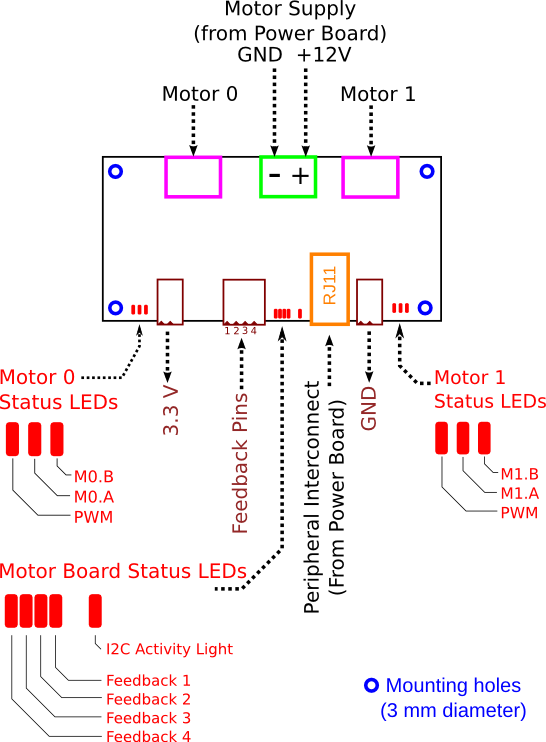
\includegraphics[scale=1]{outline}
\caption{1:1 Scale Drawing of the Motor Board}
\end{figure}

\section{Connecting it up}
The motor controller has the following inputs and outputs.
\begin{enumerate}
\item \textbf{RJ11 -- Logic Power and Data:} Connects RJ11 Socket on Power Board to RJ11 Socket on Motor Board  
\item \textbf{Motor supply:} A Student Robotics Connector delivers power from the Power Board's `12V Motor Supply' to the Motor Board
\item \textbf{Motor outputs:} Student Robotics Connectors are used to connect the terminals of the motors to the Motor Board. 
\item \textbf{Feedback inputs:} See future feedback documentation 
\item \textbf{3.3 V Supply:} For use with external, optional feedback circuitry
\item \textbf{Ground Connection:} For use with external, optional feedback circuitry
\end{enumerate}

Some technical information about the types of motor which the Motor Board supports is detailed in table \ref{tab:numspecs}
\begin{table}[h]
  \caption{\label{tab:numspecs}Specifications of the motor controller.}
  \begin{center}
    \begin{tabular}{|l|c|c|}
      \hline
      \textbf{Description} & \textbf{Value} & \textbf{Units} \\
      \hline
      Maximum supply voltage (V$_M$) & 14.5 & V \\
      Output motor & $V_M - 0.4$ & V \\
      Maximum output current & 3.5 & A \\
      \hline
    \end{tabular}
  \end{center}
\end{table}

\section{LED Indicators}
The motor controller has three banks of LEDs. The two outer banks describe the state of the two motor outputs. The leftmost (as viewed in figure \ref{fig:outline} represents Motor 0, and the rightmost, Motor 1. Together `MX.A' \& `MX.B' describe the direction of the motor:


\begin{table}[h]
	\caption{\label{tab:statusleds}Motor States}
	\begin{center}
		\begin{tabular}{|l|c|c|}
			\hline
			MX.A & MX.B & Status \\ 
			\hline
			0 & 0 & Forward \\
			0 & 1 & Backward \\
			1 & 0 & Brake \\
			1 & 1 & Off \\
			\hline		
		\end{tabular}
	\end{center}
\end{table}

The PWM LEDs give a visual indication of the speed of the motors. The brighter the LED the more power is being delivered to the motor. This may be useful when testing your robot in Charge mode, since the motor power rail is disabled.


\section{Feedback}
Motor feedback allows the Motor Board to maintain a constant and known speed, regardless of factors such as wheels slipping and resistance due to other robots or obstacles. It also allows you to keep track of the distance you have travelled.  

\vspace{12pt}

\noindent {\bf NOTE: Support for Motor Feedback will be introduced after the Electronics Release day via the IDE. More information will be made available in the near future}

\vspace{12pt}

The motor controller will support the following methods of feedback:
\begin{itemize}
\item Quadrature (2-bit) Rotary Encoder with Gray coding. See `Incremental rotary encoder' section on Wikipedia:  http://en.wikipedia.org/wiki/Rotary\_encoder
\item Single bit tachometer (cannot detect direction) 
\end{itemize} 

3.3V and GND connections are supplied on the Motor Board to make it easier to connect the switches and sensors necessary for feedback.

\vspace{12pt}

\noindent {\bf More information about how to make use of Motor Feedback will be made available after its implementation} 


\end{document}
